\documentclass[11pt, oneside]{article}   	% use "amsart" instead of "article" for AMSLaTeX format
\usepackage{geometry}                		% See geometry.pdf to learn the layout options. There are lots.
\geometry{letterpaper, margin=1in}                   		% ... or a4paper or a5paper or ... 
%\geometry{landscape}                		% Activate for rotated page geometry
%\usepackage[parfill]{parskip}    		% Activate to begin paragraphs with an empty line rather than an indent
\usepackage{graphicx}				% Use pdf, png, jpg, or eps§ with pdflatex; use eps in DVI mode
								% TeX will automatically convert eps --> pdf in pdflatex		
\usepackage{amssymb}


\title{MCSC 6030G : High Performance Computing \\ Assignment 1: Matrix-Vector Product}
\author{Parikshit Bajpai \\ 100693928}
\date{}							% Activate to display a given date or no date

\begin{document}
\maketitle

\section{Introduction}
Computing, in today's world, has radically changed since the days of Konrad Zuse who constructed the world's first fully automated, freely   programmable computer with binary floating-point arithmetic in 1941 \cite{Rojas:2002aa}.  Zuse's  great visions regarding the possible use of his device are now a reality, and computers, owing to their computational abilities at an incredible, ever-increasing speed, have become essential, not only in science and engineering but in all sectors of life \cite{Zuse:1993aa}.

As an essential tool for most research areas, both in academia and industry, computer-based simulations have become ever-present standard tools. However, even with the rapid increase in the performance of desktop machines, there still remain tasks with requirements on raw computational speed, storage, or main memory which require dedicated computational frameworks \cite{Hager:2010aa}. High Performance Computing, in general, refers to the practice of clustering computing power in a way that delivers much higher performance than one could get out of a typical desktop computer or workstation in order to solve large problems in science, engineering, or business \cite{insidehpc:aa}.

In times of stagnating single processor capabilities and increasing parallelism, there has been a growing focus on the performance and scalability, and the most sensible measure of performance in benchmarking is the \textit{wallclock time}, also called \textit{elapsed time} \cite{Hager:2010aa}. In order to reduce wallclock times, HPC systems rely on a few techniques such as parallelisation, compiler optimisation, and use of standard libraries.

Parallel processing refers to processing the program instructions by splitting them into multiple threads in order to reduce execution time. The different threads can perform different subtasks simultaneously thus reducing the time required for the execution. OpenMP is a shared memory parallel programming API that works on the fork-join model and consists of a set of compiler directives that a non-OpenMP-capable compiler would just regard as comments and ignore \cite{Board:2015aa}. In context of parallelisation, apart from the wallclock time, the following parameters are of interest:
\begin{equation} \label{Speedup}
Speed \: Up = \frac{Serial \: Wall \: Time}{Parallel \: Wall \: Time} = \frac{S}{P}
\end{equation}
\begin{equation} \label{Efficiency}
Efficiency = \frac{Speed  \: Up}{Number \: of  \: Threads} = \frac{S}{n \times P}
\end{equation}

Apart from parallelisation, optimising compilers has become an essential component of modern high-performance computer systems. In addition to translating the input program into machine language, the compilers analyse it and apply various transformations to reduce its running time or its size \cite{Bacon:1994aa}. Amongst the popular compilers, GNU Gfortran has developed an open-source \textit{gfortran} compiler capable of working on multiple architectures and diverse environments, and, Intel has developed the \textit{ifort} compiler to deliver superior Fortran application performance and to boost Single Instruction Multiple Data (SIMD) vectorisation and threading capabilities \cite{Corporation:2018aa}.

\section{Methodology}
\subsection{Objective}
The present study is aimed at exploring the impact of code, compiler and execution on the wall time for matrix-vector multiplication problem. To this aim, compiler optimisation, parallelisation, and use of standard software library have been implemented and the wall times have been compared.

\subsection{Machine Configuration}
	\textbf{Manufacturer \& Model}: Lenovo ThinkPad Yoga 370\\
	\textbf{Processor}: Intel Core i5 -7200U (4 processor cores)\\
	\textbf{Clock Rate}:  2.50 GHz\\
	\textbf{RAM}:  16 GB\\
	\textbf{Operating System}: Ubuntu 18.04\\
	
\subsection{Implementation}
In order to obtain a reference performance benchmark, the standard double-loop code for matrix-vector multiplication was implemented without optimisation and parallelisation and compiled using the GNU compiler \textit{gfortran}, and the matrix size for which the wall time obtained was of the order of 10 seconds was selected for further study. The matrix size corresponding to the aforementioned wall time was \(8192\times8192\). Once the matrix size was fixed, compiler optimisation, parallelisation and use of standard library was implemented and the obtained wall times were compared with that obtained for the double loop without optimisation case. For this purpose, the following primary cases and their combinations were considered:
\begin{enumerate}
	\item{Choice of compiler: GNU \textit{gfortran} or Intel \textit{ifort}}
	\item{Compiler optimisation: no optimisation (-o0) or aggressive optimisation (-o3)}
	\item{Parallelisation: 1, 2 or 3 OpenMP threads}
	\item{Matrix multiplication approach: double loop or BLAS standard library}
\end{enumerate}

The BLAS (Basic Linear Algebra Subprograms) are routines that provide standard building blocks for performing basic vector and matrix operations \cite{Blackford:2002aa} and LAPACK routines are written so that as much as possible of the computation is performed by calls to the Basic Linear Algebra Subprograms (BLAS) \cite{Lawson:1979aa}. The wall times obtained based on the above strategies used individually and in conjunction were then used to calculate the speed up and efficiency of parallelisation based on equation~\ref{Speedup} and equation~\ref{Efficiency} respectively. 

Ibrahim Guiagoussou, Marcos Machado, Celina Desbiens and myself worked together on building the codes, executing and interpreting the results. 
	
\section{Results and Discussion}
The source code was run for a number of different cases presented above and the obtained results have been presented in Figure~\ref{results}. The results highlight that the wall times obtained using the Intel compiler are significantly less than those obtained using the  GNU compiler. This can attributed to the optimisation of Intel compilers for systems using Intel processors and the high-level techniques used by the compiler to reduce stalls and produce codes that execute in the fewest possible number of cycles \cite{Corporation:2018aa}. 
	\begin{figure}[h]
		\centering
		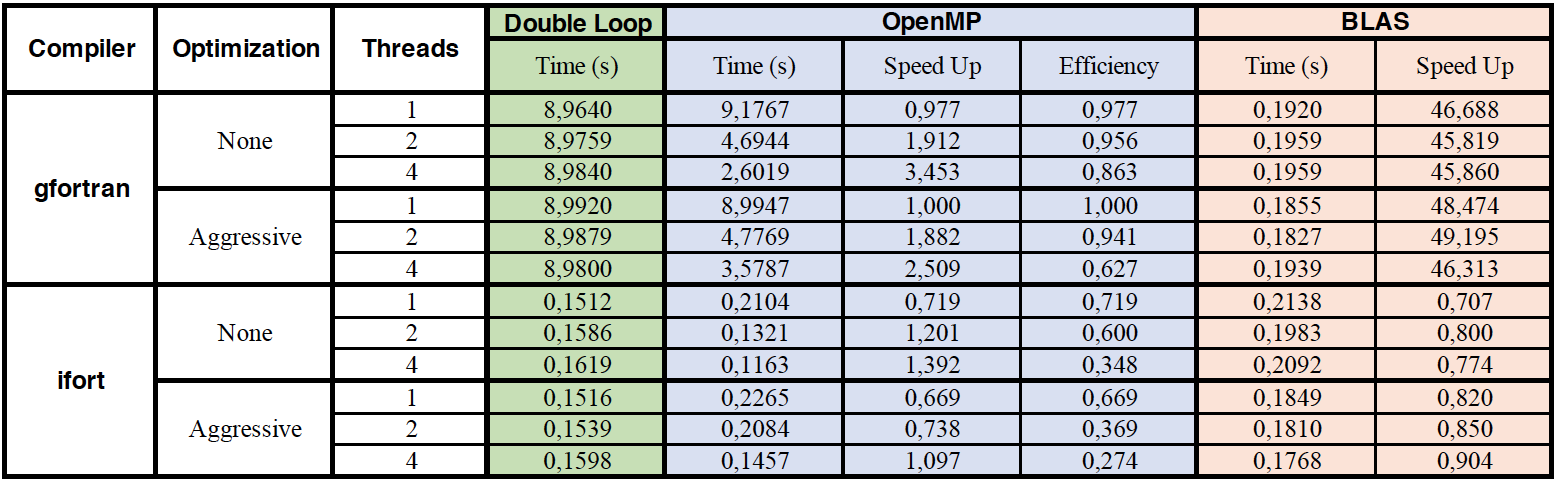
\includegraphics[width=\textwidth]{Results}
		\caption{Wall time [s], speed up and efficiency for the considered cases.}
		\label{results}
	\end{figure} 
Parallelisation was implemented using OpenMP directives and we observe a significant reduction in the wall times as the number of threads was increased. However, we also notice that the speed up did not increase linearly when the number of threads was increased from 2 to 4. Such a non-linear increase can, most probably, be attributed to increase in overheads as the number of threads is increased. Use of the BLAS library with \textit{gfortran} compiler resulted in the most significant increase in speed up. However, the wall times using OpenMP and BLAS concurrently were higher than the wall times obtained using them individually. For the sake of brevity, these results, therefore, have not been presented. They can, however, be viewed by running the shell script \textit{run.sh} in the repository.

Interestingly, when using BLAS library, we observe that the wall times achieved using \textit{gfortran} compiler were lower than those obtained using \textit{ifort} compiler. In fact, when compared with the double loop code compiled with the relevant compiler, the speed up obtained using BLAS and \textit{gfortran} compiler was around two orders of magnitude higher than the speed up obtained using BLAS and \textit{ifort}. 

\section{Conclusion}
In general, the impact of compiler optimisation, parallelisation, and use of standard library on the performance is evident from the obtained results. The results of the different cases reveal that, as foreseen, the Intel \textit{ifort} compiler is more efficient than the GNU \textit{gfortran} compiler. Furthermore, we observe that both parallelisation and use of standard library significantly speeds up the code. The tests highlight the importance of the aforementioned ways of improving the performance of codes developed for HPC and show how these can be used individually and in conjunction with each other to achieve the best possible performance from the available. computing device. 

\bibliographystyle{ieeetr}
\bibliography{Assignment_1_Parikshit}

\end{document}  